\chapter{M\"obius numbers and loops}
\label{ch:mobius}

% Part V, added 2026-09-25 from ~/Downloads/chygraph_master_equation/draft.tex,
% Sec. 10. One thing is computed, Sec. mb-computed: the loop series on the
% pairwise and the promoted factor graphs (statmech.loopseries,
% figs/loopseries.py), and the split of Ch. 14's error into double count
% and loop. The one further place the chapter goes beyond
% the draft is Sec. mb-collapse, where the draft's "exactness is
% collapsibility" is weakened to an implication, with the wheel as the
% witness that the converse fails.

Section~\ref{sec:ce-yields} ended on a promise: the counting numbers that the
Bethe free energy carries --- one per complex, one per atom, minus one per
inclusion --- were obtained in this book three times, from the replica
calculation of Sec.~\ref{sec:replicas-chy}, from the region graph of
Chapter~\ref{ch:gbp}, and from the factor graph of $\alpha+I$, and the
promise was to say what they are. They are the M\"obius function of the
inclusion order. That one sentence is the connection this chapter makes, and
the rest of the chapter is what follows from it: that their sum is an Euler
characteristic, so that exactness reads as the vanishing of a Betti number;
that the error of Part~IV is a sum over the generators of a homology group;
that the leaf removal Chapter~\ref{ch:exactness} runs on the incidence
structure is a sequence of collapses; and that the transition
Chapter~\ref{ch:exactness} found has a companion in random topology.

The field on the other side is applied topology, and the connection runs
through one author. \citet{peltre2019,peltre2020,peltre2021} write generalised belief
propagation as a flow on a cochain complex over the poset of regions, with
the counting numbers of \citet{yedidia2005} as the M\"obius function of that
poset. Everything here is that construction with the poset chosen for it: not
a family of regions given by hand, but the inclusion order of a chygraph,
which is canonical and comes with an ensemble.

\section{The counting numbers are a M\"obius function}
\label{sec:mb-mobius}
\index{M\"obius function|textbf}
\index{counting numbers|textbf}
\index{Euler characteristic|textbf}
\index{Bethe free energy}
\index{region graph}
\index{merging complexes}

Take the vertices of a chygraph, atoms and complexes alike, ordered by
inclusion. Chapter~\ref{ch:gbp}'s rule~3, Eq.~\eqref{eq:mobius}, assigns to
every element $R$ of a family closed under intersection the number
\begin{equation}
  c_{R}=1-\sum_{R'\supsetneq R}c_{R'},
  \label{eq:mb-count}
\end{equation}
working down from the maximal elements, which take $c_{R}=1$. Add a top
element $\hat1$ above everything and Eq.~\eqref{eq:mb-count} is the defining
recursion of the M\"obius function of the resulting poset, $c_{R}=-\mu(R,\hat1)$
\citep{yedidia2005}; that is what ``M\"obius inversion'' in
Chapter~\ref{ch:gbp} meant, and the recursion is how it is computed. So far
nothing is specific to chygraphs. What is specific is what happens when the
family is the inclusion order itself, with no closure taken.

\paragraph{The treelike case.} Suppose the incidence structure of
Sec.~\ref{sec:treelike} --- the bipartite graph of atoms and complexes, or
of complexes and their containers at every level --- is a forest. Let
$S(x)$ be the sum in Eq.~\eqref{eq:mb-count}, taken over every element
strictly above $x$. A vertex $x$ has $\kappa_{x}$ immediate containers
$b_{1},\dots,b_{\kappa_{x}}$, and in a forest the sets of elements above two
different containers are disjoint, since a common container of $b_{1}$ and
$b_{2}$ would close a loop $x\,b_{1}\,c\,b_{2}\,x$. So the sum splits by
container,
\begin{equation}
  S(x)=\sum_{j}\bigl[c_{b_{j}}+S(b_{j})\bigr]
      =\sum_{j}\bigl[1-S(b_{j})+S(b_{j})\bigr]=\kappa_{x},
  \label{eq:mb-forest}
\end{equation}
and therefore
\begin{equation}
  c_{x}=1-\kappa_{x}
  \qquad\text{for every vertex, atom or complex, at every depth.}
  \label{eq:mb-treecount}
\end{equation}
That is Eq.~\eqref{eq:bethe}: $1-\kappa$ on every atom, and on every complex
$1-\kappa_{a}$, which is the $+1$ of its factor together with the
$-\kappa_{a}$ of its variable that Sec.~\ref{sec:ce-yields} counted on the
factor graph of $\alpha+I$. Averaged over a layer it is $n_{l}=\ave{\kappa_{l}}/c_{l}$
complexes per atom carrying weight one, and $\ave{1-\kappa}$ on the atoms,
which are the coefficients of the two terms of Eq.~\eqref{eq:bethe} and,
term for term, the three terms of the replica free energy
Eq.~\eqref{eq:Fchy} --- one per complex, one per atom, one subtracted per
inclusion. Three derivations, one M\"obius function, and the reason the three
agreed is that each of them was computing it.

\paragraph{The sum is an Euler characteristic.} Sum
Eq.~\eqref{eq:mb-treecount} over the vertices of the incidence structure. The
number of vertices is the number of atoms plus the number of complexes, and
$\sum_{x}\kappa_{x}$ counts every inclusion once, so
\begin{equation}
  \sum_{x}c_{x}=V-E=b_{0}-b_{1},
  \label{eq:mb-euler}
\end{equation}
the Euler characteristic of the incidence graph, which for a graph is the
number of connected components less the number of independent cycles. On a
connected forest it is one. The counting numbers of the inclusion order
therefore sum to one exactly when the incidence structure has no loops,
which is the condition Sec.~\ref{sec:mergeerror} showed the chygraph
recursion itself needs: \emph{the recursion on the chygraph itself is
exact when $b_{1}=0$ of the incidence structure}, and the counting numbers
are the local quantities whose total is that Betti number. In the
hierarchy of \citet{fagin1983} that condition is \emph{Berge-acyclicity}
of the complex family, the strongest of the four he orders, and the three
names of Chapter~\ref{ch:exactness} are $\alpha$-acyclicity, the weakest;
the chain runs Berge, $\gamma$, $\beta$, $\alpha$, each implying the
next. Two triangles sharing an edge are $\alpha$-acyclic, and the
join-tree calculation is exact on them, but their incidence structure has
a loop; the next paragraph is that example, and what the two repairs of
Part~IV do to its counting numbers is exactly the difference between the
two conditions.

\paragraph{Two triangles.} The example Part~IV opened with makes the
arithmetic visible (Fig.~\ref{fig:mobiusposet}). Two triangles $a=\{1,2,3\}$
and $b=\{2,3,4\}$ share the pair $\{2,3\}$. On the inclusion order of the
chygraph, the two complexes take $c=1$, atoms $1$ and $4$ take
$1-1=0$, and atoms $2$ and $3$ take $1-2=-1$. The sum is $0$: the incidence
graph has six vertices and six inclusions, and the loop $2\,a\,3\,b\,2$ is its
one independent cycle. The bond $(2,3)$ is inside both complexes and is
counted twice, which is the double count of Sec.~\ref{sec:twotriangles}, and
the sum of the counting numbers has recorded the fact before any free energy
is evaluated.

Both repairs of Part~IV restore the sum to one, from opposite sides, and
they restore it to different objects.
Chapter~\ref{ch:gbp} closes the family under intersection, inserting the pair
$\{2,3\}$ as an element of the order. Its counting number is $1-2=-1$, and
the atoms below it now have $1-(1+1-1)=0$; the sum is $1+1-1=1$, and the
Hasse diagram of the closed family, with seven elements and six covering
relations, is a tree. That is Fig.~\ref{fig:regiongraph} read as a poset.
Chapter~\ref{ch:metacomplex} instead merges the two triangles into one
complex $\{1,2,3,4\}$, which takes $c=1$ while every atom takes $0$; the sum
is again one, and the incidence structure is a star. One repair adds an
element below the loop and the other removes the loop by replacing its two
complexes with one; either way the sum returns to one, and the counting
numbers say so before either calculation is run. The two are not the same
condition. The closed family's Hasse diagram is a tree here and need not be
in general --- three cliques in a path, $\{1,2,3\}$, $\{2,3,4\}$,
$\{3,4,5\}$, close to a family in which atom $3$ lies below two separators
and the diagram has a cycle, while the family is chordal, the calculation is
exact and the counting numbers still sum to one, three cliques less two
separators. On a junction tree the sum is always cliques minus separators,
which is one; what the sum reads on the closed family is the join-tree
condition of Chapter~\ref{ch:exactness}, and what it reads on the inclusion
order itself is the forest condition of Chapter~\ref{ch:metacomplex}.

\begin{figure}[t]
\centering
\begin{adjustbox}{width=0.97\linewidth}
\begin{tikzpicture}[x=1cm,y=1cm]
% ---- left: the inclusion order of the chygraph ----
\begin{scope}
  \node[atm] (p1) at (0,0) {};
  \node[atm] (p2) at (0.9,0) {};
  \node[atm] (p3) at (1.8,0) {};
  \node[atm] (p4) at (2.7,0) {};
  \node[cpx] (A) at (0.9,1.4) {};
  \node[cpx] (B) at (1.8,1.4) {};
  \draw[inc] (p1)--(A) (p2)--(A) (p3)--(A);
  \draw[inc] (p2)--(B) (p3)--(B) (p4)--(B);
  \node[lb,below=1pt of p1] {$0$};
  \node[lb,below=1pt of p2] {$-1$};
  \node[lb,below=1pt of p3] {$-1$};
  \node[lb,below=1pt of p4] {$0$};
  \node[lb,above=1pt of A] {$1$};
  \node[lb,above=1pt of B] {$1$};
  \node[lb,left=2pt of A] {$a$};
  \node[lb,right=2pt of B] {$b$};
  \node[tb,anchor=north,align=center] at (1.35,-0.55)
    {inclusion order\\ $\sum c=0$, $b_{1}=1$};
\end{scope}
% ---- middle: closed under intersection (the region graph) ----
\begin{scope}[xshift=4.6cm]
  \node[atm] (p1) at (0,0) {};
  \node[atm] (p2) at (0.9,0) {};
  \node[atm] (p3) at (1.8,0) {};
  \node[atm] (p4) at (2.7,0) {};
  \node[cpxb] (S) at (1.35,0.8) {};
  \node[cpx] (A) at (0.7,1.7) {};
  \node[cpx] (B) at (2.0,1.7) {};
  \draw[inc] (p1)--(A) (p2)--(S) (p3)--(S) (p4)--(B);
  \draw[inc] (S)--(A) (S)--(B);
  \node[lb,below=1pt of p1] {$0$};
  \node[lb,below=1pt of p2] {$0$};
  \node[lb,below=1pt of p3] {$0$};
  \node[lb,below=1pt of p4] {$0$};
  \node[lb,right=2pt of S] {$-1$};
  \node[lb,above=1pt of A] {$1$};
  \node[lb,above=1pt of B] {$1$};
  \node[tb,anchor=north,align=center] at (1.35,-0.55)
    {closed under intersection\\ $\sum c=1$, $b_{1}=0$};
\end{scope}
% ---- right: merged ----
\begin{scope}[xshift=9.2cm]
  \node[atm] (p1) at (0,0) {};
  \node[atm] (p2) at (0.9,0) {};
  \node[atm] (p3) at (1.8,0) {};
  \node[atm] (p4) at (2.7,0) {};
  \node[cpx] (M) at (1.35,1.4) {};
  \draw[inc] (p1)--(M) (p2)--(M) (p3)--(M) (p4)--(M);
  \node[lb,below=1pt of p1] {$0$};
  \node[lb,below=1pt of p2] {$0$};
  \node[lb,below=1pt of p3] {$0$};
  \node[lb,below=1pt of p4] {$0$};
  \node[lb,above=1pt of M] {$1$};
  \node[tb,anchor=north,align=center] at (1.35,-0.55)
    {merged\\ $\sum c=1$, $b_{1}=0$};
\end{scope}
\end{tikzpicture}
\end{adjustbox}
\caption{\textbf{The counting numbers as a M\"obius function.} Two triangles
sharing the pair $\{2,3\}$, drawn as inclusion orders with the number
Eq.~\eqref{eq:mb-count} assigns written at each element. Left: the chygraph
itself. The shared atoms carry $-1$, the sum is zero, and the incidence
graph has one independent cycle. Middle: the family closed under
intersection, Chapter~\ref{ch:gbp}'s region graph, with the shared pair
(shaded) inserted below the two triangles carrying $-1$; the Hasse diagram is
a tree and the sum is one. Right: the merge closure of
Chapter~\ref{ch:metacomplex}, one complex on four atoms, a star, sum one.
The sum is the Euler characteristic of the incidence structure,
Eq.~\eqref{eq:mb-euler}, so it reads the loop before any free energy does,
and both repairs of Part~IV are ways of removing it.}
\label{fig:mobiusposet}
\end{figure}

\section{The loop series}
\label{sec:mb-loops}
\index{loop series|textbf}
\index{generalised loop}

If exactness is $b_{1}=0$, the error when $b_{1}>0$ ought to be organised by
the generators of $H_{1}$, and it is. \citet{chertkov2006} expand the
partition function of a model on a factor graph around the belief-propagation
fixed point,
\begin{equation}
  Z=Z_{\mathrm{BP}}\Bigl(1+\sum_{C}r_{C}\Bigr),
  \label{eq:mb-loopseries}
\end{equation}
the sum running over the \emph{generalised loops} of the factor graph --- the
subgraphs in which no vertex has degree one --- with each term $r_{C}$ a
product over the vertices of $C$ of connected correlations evaluated at the
fixed point. A tree has no generalised loop and the series is the single term
one, which is exactness again. On the factor graph of $\alpha+I$ the
generalised loops are the loops \emph{over complexes}, and the series is the
natural home for the error terms Part~IV measured one at a time.

\paragraph{The one-loop term.} The ring of $k$ triangles glued at single
atoms, Fig.~\ref{fig:ring}, is the smallest object on which the series has
exactly one term beyond the leading one. Its incidence structure is a single
cycle of $2k$ steps, so $b_{1}=1$ and there is one generalised loop, the ring
itself. Table~\ref{tab:ring} measured the error of the cavity method on it at
$k=4$ to $8$ and found it falling with $k$ at fixed coupling, a short-loop
effect and not a defect of the scheme. In Eq.~\eqref{eq:mb-loopseries} that
is the statement that $r_{C}$ for the one loop is a product of $2k$ factors
each less than one in magnitude, and the rate at which the error falls with
$k$ is the logarithm of the typical factor. The book did not compute
$r_{C}$; Table~\ref{tab:ring} measured $Z$ and $Z_{\mathrm{BP}}$ and took
the difference, and the loop series says what that difference is a series
in.

\paragraph{Motif promotion is a partial resummation.} Here is the claim the
connection makes, and it is a concrete one. A graph rich in triangles has, on
its own factor graph, a generalised loop for every triangle and for every
combination of triangles, and the loop series of the graph is a sum over all
of them. Promote each triangle to a complex, as Sec.~\ref{sec:promoting}
does, and the triangle is a single factor of $\alpha+I$: the loop that ran
around its three edges is now \emph{inside} a factor, and it is not a
generalised loop of the new factor graph at all. Its contribution has not
been dropped. It has been summed exactly by the interior sum, Eq.~\eqref{eq:emitted},
which is where Chapter~\ref{ch:statmech} said the loops went. So the chygraph
recursion on a clique chygraph is, in the language of
Eq.~\eqref{eq:mb-loopseries}, the loop series of the graph with every
generalised loop that lives inside a single clique resummed into the leading
term, and the remaining series runs only over loops between cliques.
Two things should be kept apart here. On two triangles sharing an edge
the factor graph of $\alpha+I$ has exactly one generalised loop, the loop
$2\,a\,3\,b\,2$ of Fig.~\ref{fig:mobiusposet}, and
Eq.~\eqref{eq:mb-loopseries} is an identity on any finite factor graph, so
$Z/Z_{\mathrm{BP}}-1=r_{C}$ is guaranteed to reproduce
Table~\ref{tab:twotriangles}; computing it is a check of arithmetic, not
a test. The claim that needs testing is the one above: that the loop
series of the promoted factor graph is the loop series of the pairwise
graph with every intra-clique loop resummed. That is not a term-by-term
correspondence --- the two expansions are around different fixed points,
and the four-cycle $1\,2\,4\,3$ of the pairwise graph has no single image
in the promoted series --- and whether it holds as a statement about the
two sums is what would be tested on the objects Part~IV already holds. Section~\ref{sec:mb-computed} runs both series, and finds something the
question did not anticipate.


\section{The series, computed}
\label{sec:mb-computed}
\index{loop series!computed|textbf}
\index{double counting}

Everything in the previous section is now measured, and the measurement
turns one of Part~IV's findings around.
\code{statmech.\allowbreak loopseries} enumerates the generalised loops of a
binary factor graph by backtracking over its factors, evaluates each term
of Eq.~\eqref{eq:mb-loopseries} from the belief-propagation fixed point,
and compares $\ln(1+\sum_{C}r_{C})$ with $\ln Z-\ln Z_{\mathrm{BP}}$ from
exact enumeration. The identity holds to $10^{-15}$ on every factor graph
tried, a triangle (where the one term is $\tanh^{3}\beta J$), two
triangles sharing an edge, rings of four to six triangles and a random
graph, on the pairwise factor graph and on the promoted one alike. The
promoted factor graph is the one thing that has to be said precisely
before any of this is run. The factor graph of $\alpha+I$ represents the
Ising model only if every bond enters exactly one complex's kernel; where
two cliques share an edge the kernel of one of them must leave that bond
out. The chygraph recursion of Chapter~\ref{ch:overlap} gives both cliques
the bond, which is a different model, and Chapter~\ref{ch:overlap} measured
the recursion's error against the true $Z$. The loop series sorts that
error into two parts, and the sorting is the result of this section.

\paragraph{Rings.} Table~\ref{tab:loopseries-ring} is the ring of $k$
triangles of Fig.~\ref{fig:ring} on both factor graphs. On the promoted one
the series has one term, the ring itself, and it reproduces
Table~\ref{tab:ring}'s error to the last digit, which is the arithmetic
check Sec.~\ref{sec:mb-loops} promised. On the pairwise one the series has
$103$, $323$ and $1019$ terms at $k=4$, $5$, $6$; its leading terms, the
triangles, carry $0.81$ to $0.92$ of the whole at $\beta J=0.3$ and $0.32$
to $0.36$ at $0.8$, and the partial sums reach one per cent of the whole
only at loops of twelve to fourteen legs at the weak coupling and eighteen
to twenty-four at the strong one (Fig.~\ref{fig:loopseries}a). The two
expansions are around different fixed points, and the promoted one starts
closer: its single term is $0.018$ against a pairwise error of $0.116$ at
$k=4$ and $\beta J=0.3$, and $0.0024$ against $0.149$ at $k=6$, the ring
loop weakening with the ring's length while the pairwise error grows with
the number of triangles. That is the resummation of
Sec.~\ref{sec:mb-loops} in the one case where it can be seen whole: every
loop inside a triangle is gone from the promoted series, and what remains
is the one loop between the triangles.

\begin{table}[tb]
\centering\small
\begin{adjustbox}{max width=\linewidth}
% generated by figs/loopseries.py; do not edit
\begin{tabular}{rrrrrrrr}
\hline\hline
$k$ & $n$ & $\beta J$ & \multicolumn{4}{c}{pairwise} & promoted\\
 & & & loops & error & triangles & size at $1\%$ & error\\
\hline
4 & 8 & 0.3 & 103 & 0.1157 & 0.81 & 12 & 0.0180\\
4 & 8 & 0.8 & 103 & 1.4549 & 0.36 & 18 & 0.4277\\
5 & 10 & 0.3 & 323 & 0.1287 & 0.90 & 14 & 0.0066\\
5 & 10 & 0.8 & 323 & 1.6599 & 0.34 & 20 & 0.3758\\
6 & 12 & 0.3 & 1019 & 0.1490 & 0.92 & 14 & 0.0024\\
6 & 12 & 0.8 & 1019 & 1.8701 & 0.32 & 24 & 0.3292\\
\hline\hline
\end{tabular}

\end{adjustbox}
\caption{\textbf{The loop series on a ring of $k$ triangles, both factor
graphs.} For the pairwise factor graph: the number of generalised loops,
the error $\ln Z-\ln Z_{\mathrm{BP}}$, the share of $\sum_{C}r_{C}$ carried
by the triangles alone, and the loop size at which the partial sum is
within one per cent of the whole. For the promoted factor graph the series
has one term, whose value is the error in the last column, and it is
Table~\ref{tab:ring}'s. \code{figs/\allowbreak loopseries.\allowbreak py}.}
\label{tab:loopseries-ring}
\end{table}

\begin{figure}[tp]
\centering
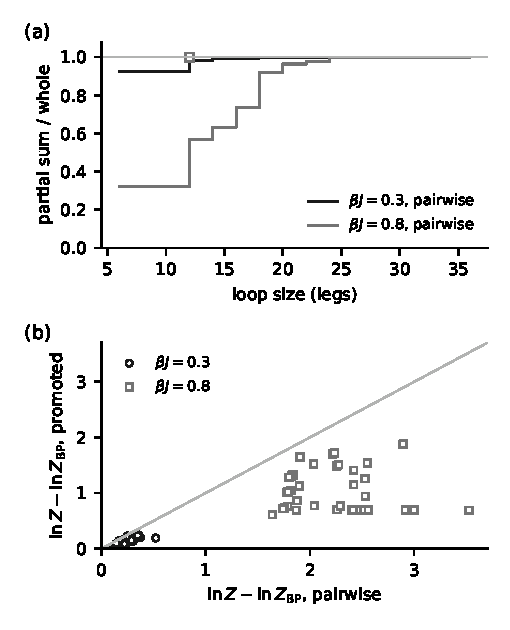
\includegraphics[width=0.8\linewidth]{figs/fig-loopseries.pdf}
\caption{\textbf{Two factor graphs, two series.} (a) Partial sums of the
pairwise loop series on a ring of six triangles, by loop size, as a
fraction of the whole; the markers at twelve legs are the promoted series,
which is one term. (b) Forty clustered instances --- ten atoms, four
triangles placed at random and three further edges --- at two couplings:
the error of belief propagation on the pairwise factor graph against the
error on the promoted one with every bond in one clique. Every point lies
below the diagonal. \code{figs/\allowbreak loopseries.\allowbreak py}.}
\label{fig:loopseries}
\end{figure}

\paragraph{Clustered instances.} Figure~\ref{fig:loopseries}b puts the same
comparison on forty instances small enough to enumerate exactly: ten atoms,
four triangles placed at random, three further edges, so that triangles
share atoms and edges and the maximal cliques are what
Chapter~\ref{ch:data} would extract. The pairwise series has $814$ terms on
average, the promoted one $285$; the pairwise error is $0.23$ at
$\beta J=0.3$ and $2.24$ at $0.8$, the promoted one $0.14$ and $1.10$, and
the promoted error is the smaller on every one of the forty at both
couplings. So the claim of Sec.~\ref{sec:mb-loops} holds in the form it was
stated in after the review: not term by term, since the two series expand
around different fixed points, but as a statement about the two sums --- the
promoted series is shorter, and it has less to do.

\paragraph{What Part~IV's error was.} The chygraph recursion of
Chapter~\ref{ch:overlap} is belief propagation on the factor graph of
$\alpha+I$ with every clique given every bond inside it. Its error against
the true $\ln Z$ therefore splits exactly in two,
\begin{equation}
  \ln Z^{\mathrm{dc}}_{\mathrm{BP}}-\ln Z
  =\bigl(\ln Z^{\mathrm{dc}}-\ln Z\bigr)
  +\bigl(\ln Z^{\mathrm{dc}}_{\mathrm{BP}}-\ln Z^{\mathrm{dc}}\bigr),
  \label{eq:mb-decomposition}
\end{equation}
the first bracket the double count --- the exact partition function of the
doubled Hamiltonian against that of the true one --- and the second the
loop series of the doubled model's factor graph, which is what belief
propagation itself gets wrong. Table~\ref{tab:loopseries-dc} evaluates both
on the two triangles of Table~\ref{tab:twotriangles} and on twenty
hyperbolic instances of fourteen atoms with overlapping cliques, drawn
afresh from the ensemble of Chapter~\ref{ch:overlap}. The two parts have
opposite signs on every instance. On two triangles at $\beta J=0.5$ the
recursion's error of $+0.09$ is $+0.41$ of double count against $-0.32$ of
loop; on the hyperbolic instances the double count is $+2.0$ against
$-0.7$ at $\beta J=0.3$ and $+6.3$ against $-0.7$ at $0.8$, larger than the
loop part on nineteen of twenty and on all twenty. What
Chapter~\ref{ch:overlap} measured as the price of treelikeness is, on
these instances, mostly not a loop effect at all: it is the bond counted
twice, and the loop part is a fraction of it that does not grow with the
coupling.

\begin{table}[tb]
\centering\small
\begin{adjustbox}{max width=\linewidth}
% generated by figs/loopseries.py; do not edit
\begin{tabular}{lrrrrr}
\hline\hline
instance & $\beta J$ & recursion & double count & loop & assigned once\\
\hline
two triangles & 0.2 & $+0.0184$ & $+0.0720$ & $-0.0535$ & $-0.0091$\\
two triangles & 0.5 & $+0.0908$ & $+0.4116$ & $-0.3208$ & $-0.1234$\\
two triangles & 1.0 & $+0.3680$ & $+0.9918$ & $-0.6238$ & $-0.4316$\\
two triangles & 2.0 & $+1.3082$ & $+2.0000$ & $-0.6918$ & $-0.6565$\\
hyperbolic $n=14$, mean of 20 & 0.3 & $+1.2921$ & $+2.0224$ & $-0.7303$ & $-0.4113$\\
hyperbolic $n=14$, mean of 20 & 0.8 & $+5.5387$ & $+6.2701$ & $-0.7314$ & $-0.9067$\\
\hline\hline
\end{tabular}

\end{adjustbox}
\caption{\textbf{The recursion's error, split by
Eq.~\eqref{eq:mb-decomposition}.} Columns: the error of the chygraph
recursion of Chapter~\ref{ch:overlap} against the true $\ln Z$; its
double-count part; its loop part; and, for comparison, the error of belief
propagation on the same factor graph with every bond assigned to one
clique. Two triangles sharing an edge at the couplings of
Table~\ref{tab:twotriangles}, and the mean over twenty hyperbolic
instances of fourteen atoms with overlapping cliques.
\code{figs/\allowbreak loopseries.\allowbreak py}.}
\label{tab:loopseries-dc}
\end{table}

The last column of the table is the cheapest repair in Part~IV, and it was
not among the three. Assign each bond to one of the cliques that contain it
and run the same recursion: no region graph, no merging, the same messages
on the same incidence structure with one kernel changed. On the hyperbolic
instances that cuts the mean error by a factor of three at $\beta J=0.3$
and six at $0.8$, and it is the smaller error on fifteen and nineteen of
the twenty. What is left is the loop part proper, the Berge loops of
Sec.~\ref{sec:mb-mobius} that no kernel assignment removes; on two
triangles at weak coupling it is larger than the recursion's error, because
there the recursion's two parts happen to cancel, which the table shows and
Chapter~\ref{ch:overlap} could not have. Chapter~\ref{ch:gbp}'s region
graph and Chapter~\ref{ch:metacomplex}'s merging both remove the double
count and the loop together, at their respective costs; the assignment
removes the double count alone, for nothing, and leaves the loop series to
say what remains.

\section{Collapsibility}
\label{sec:mb-collapse}
\index{collapsibility|textbf}
\index{GYO reduction}

Chapter~\ref{ch:exactness}'s certificate is the GYO reduction, Sec.~\ref{sec:threenames}:
delete an atom that lies in one complex only, delete a complex contained in
another, repeat, and the family is $\alpha$-acyclic if and only if nothing
is left. Read the family as a simplicial complex --- every complex a facet,
every subset of a complex a face --- and the two rules are two things a
topologist already has a name for.

An atom that lies in one complex only is a vertex whose star is a single
simplex, and removing it is a sequence of \emph{elementary collapses}: each
face of that simplex containing the vertex is a free face of the face one
dimension up, and can be removed together with it without changing the
homotopy type. A complex contained in another is a face of a facet, and
removing it from the \emph{family} changes nothing in the simplicial complex
at all, since every face of a facet is present already. So a GYO reduction
that empties the family is a sequence of elementary collapses that reduces
the simplicial complex to a point: \emph{an $\alpha$-acyclic family is
collapsible}. Collapsibility is stronger than contractibility, and it is
combinatorial, decided by a finite sequence of moves rather than by a
homotopy, which is what makes it a certificate.

The converse fails, and the draft this part grew out of stated the
equivalence; the statement here is the implication, for a reason the book
has already met. A wheel with four spokes, the hub joined to every vertex of
a four-cycle, has as its clique family the four triangles at the hub. GYO
cannot start: every atom lies in two triangles and no triangle is contained
in another, so the family is not $\alpha$-acyclic, which is why
Sec.~\ref{sec:threenames} named the wheel as a structure the join tree
cannot handle. But its simplicial complex is a cone over the rim, a disc,
and a disc is collapsible. So the residue of Sec.~\ref{sec:residue} --- what
GYO cannot consume --- is an obstruction to a join tree and not to a collapse;
the two conditions agree when they are both zero and differ on the wheel,
and it is the join-tree condition that the recursion needs. What
collapsibility does supply is a direction. The three conditions this part
has met are strictly ordered: $b_{1}=0$ of the incidence structure,
Berge-acyclicity, which Sec.~\ref{sec:mb-mobius} showed is what the
chygraph recursion itself needs, implies $\alpha$-acyclicity, since an
incidence forest is its own join tree; $\alpha$-acyclicity implies collapsibility, by the argument
above; and neither converse holds, two triangles sharing an edge separating
the first pair and the wheel the second.

\section{Random topology}
\label{sec:mb-random}
\index{acyclicity percolation}
\index{random simplicial complex|textbf}

Chapter~\ref{ch:exactness} turned ``is the family acyclic'' into a question
about an ensemble and found a transition: the vertices on short chordless
cycles, Eq.~\eqref{eq:phishort}, form finite islands at low density and a
giant piece above a threshold $\ave{k}_{a}$ that lies well above the graph's
own percolation threshold, Figs.~\ref{fig:acyclicity} and~\ref{fig:fss}.
That transition has stood alone in the book. In random topology it has a
family.

\citet{linial2006} take the complete graph on $n$ vertices, add each
triangle independently with probability $p$, and ask when the first homology
of the resulting $2$-complex vanishes; the threshold is at $p$ of order
$\ln n/n$, the two-dimensional version of the connectivity threshold of a
random graph. \citet{aronshtam2013} ask the sparser question, $p=c/n$, and
find thresholds in $c$ for collapsibility and for the vanishing of the top
homology, which do not coincide, the complex ceasing to be collapsible
before its top homology appears; \citet{kahle2014} surveys the subject.
Those are uniform faces on a complete vertex set: every $d$-simplex is
equally likely. The chygraph is the heterogeneous, layered and nested version
of the same object, with a cardinality distribution in place of a fixed $d$
and a chy-degree distribution in place of a fixed $p$, and its thresholds are
fixed by the four moment matrices of Eq.~\eqref{eq:moments} rather than by a
single constant. Acyclicity percolation is the first of those thresholds,
and it is a threshold of a different kind from Linial--Meshulam's: not where
a homology group vanishes, but where the set on which the local homology is
non-trivial percolates, which is the question a cavity method asks and a
topologist has had no reason to.

\paragraph{What the two sides share.} The collapsibility threshold of
\citet{aronshtam2013} and acyclicity percolation both sit in the sparse
r\'egime, a bounded number of faces at an edge, and both sit above a
percolation threshold of the faces themselves. For the random $2$-complex
the underlying graph is complete, so the comparison is not with its giant
component but with the giant component of triangles adjacent along shared
edges: each edge lies in a Poisson number of triangles of mean $c$ and each
triangle opens two new edges, so that giant appears at $c=1/2$, below the
collapsibility threshold near $2.46$. On the chygraph side the loss of
$\alpha$-acyclicity sits above the graph's own giant component in the
same way. That is as far as the analogy has been carried. Whether the collapsibility threshold of a
random complex is a percolation of non-collapsible islands in the same sense
as Chapter~\ref{ch:exactness}'s $\ave{k}_{a}$, and whether the layered
thresholds reduce to theirs on the uniform ensemble, are questions the
present book leaves open.

\section{Sheaf Laplacians}
\label{sec:mb-sheaf}
\index{sheaf!Laplacian|textbf}

The connection has so far been to the free energy and to exactness. The
linearised recursion, the threshold tensor of Sec.~\ref{sec:threshold} and
the branching matrix of Eq.~\eqref{eq:branch}, has its own topological
reading. \citet{hansen2019} attach to a cell complex a \emph{cellular sheaf}:
a vector space on every cell, the stalk, and a linear restriction map from a
cell to each cell in its boundary, and define the sheaf Laplacian
$L=\delta^{\top}\delta$ built from those maps. Its kernel is the space of
\emph{harmonic sections}, assignments to the cells that agree with one
another under every restriction, and its spectral gap measures how far the
sheaf is from admitting one.

Put the message spaces on the incidence structure. A directed inclusion
carries a message space, the tangent space at the trivial fixed point of the
law on that inclusion, and the kernel derivatives of Eq.~\eqref{eq:ownleg}
--- $u'_{l}$ on a member leg, $\hat u'_{l}$ on a complex's own leg --- are
the maps that carry a perturbation from one inclusion to the next through
the interior of a complex. Those are restriction maps, and a harmonic
section is a consistent local assignment: a perturbation of the messages
that every complex reproduces, which is a marginal direction of the
recursion. The threshold is where such a direction first exists, which is
the statement $\lambda=1$ of Eq.~\eqref{eq:Lambdalambda}.

One thing has to be said precisely, because the draft said it loosely. The
linearised recursion itself is not a Laplacian: it is the weighted
non-backtracking operator of the incidence graph, one entry for each pair of
consecutive directed inclusions, with the kernel derivatives as weights, and
it is not symmetric. The sheaf Laplacian is the symmetric operator built from
restriction maps that go from a cell to its cofaces, vertex to edge on the
incidence graph, whereas the kernel derivative carries a perturbation from
one directed inclusion to the next through a vertex. For the two to come
from one sheaf the kernel derivative has to factor through the stalk at the
vertex, $F(j\to a)\to F(a)\to F(a\to i)$, which is exactly the statement
that a perturbation passes through the complex's own state; where the
complex has no state that factorisation is the claim to be checked, and
until it is the connection is an analogy. What is in print is the pairwise
case: \citet{watanabe2009} prove that the linearised belief-propagation
operator and the Hessian of the Bethe free energy are related through a
weighted graph zeta function, the weighted Ihara--Bass identity, and
\citet{saade2014} use the same identity to read the stability of the
fixed point off the Bethe Hessian. That is the closest thing to the
programme of this section already carried out, on factor graphs with
pairwise factors, and it is the result the chygraph version would
generalise. So the claim is not that
Eq.~\eqref{eq:branch} \emph{is} a sheaf Laplacian, but that both are
determined by one sheaf --- stalks the message spaces, restriction maps the
kernel derivatives --- and that the threshold, a property of that sheaf, is
readable from either. A random chygraph makes it a random sheaf, an object
\citet{hansen2019} define and do not randomise; the four moment matrices
would then fix the expected spectral gap, and the transition of every
chapter in Parts~II and~III would be the closing of that gap.

\section{What it gives the book}
\label{sec:mb-gives}

Three things, in decreasing order of how settled they are.

\emph{One sentence in place of three derivations.} The counting numbers of
Eqs.~\eqref{eq:bethe}, \eqref{eq:Fchy} and~\eqref{eq:mobius} are the
M\"obius function of the inclusion order, and they were bound to agree. Their
sum over the inclusion order is the Euler characteristic of the incidence
structure, so the condition under which the chygraph recursion itself is
exact, Chapter~\ref{ch:metacomplex}'s forest, has a name, $b_{1}=0$; the
weaker condition of Chapter~\ref{ch:exactness} is read off the same
numbers on the closed family, and the two repairs of Part~IV are the two
ways of returning the sum to one that Fig.~\ref{fig:mobiusposet} draws.

\emph{A systematic expansion for Part~IV, and a correction to it.} The
loop series of Eq.~\eqref{eq:mb-loopseries} organises the corrections
that Chapters~\ref{ch:overlap} to~\ref{ch:metacomplex} measured case by
case, with the ring of Table~\ref{tab:ring} as its one-loop term and
motif promotion as a shorter series around a closer fixed point,
Sec.~\ref{sec:mb-computed}. The same calculation splits the recursion's
error into a double count and a loop part, Eq.~\eqref{eq:mb-decomposition},
and finds the double count the larger on the overlapping instances: what
Part~IV paid for was mostly the bond counted twice, and assigning each
bond to one clique recovers most of it for nothing.

\emph{A companion for the acyclicity transition.} It is no longer the only
transition of its kind: the thresholds of \citet{linial2006} and
\citet{aronshtam2013} are the uniform case of the same question, and the
chygraph is their heterogeneous and nested generalisation, with a
percolation question they have not asked.

\section{What the field could get}
\label{sec:mb-field}

Peltre's region poset is given by hand, and every application of
generalised belief propagation chooses its regions. The chygraph gives a
canonical poset from data, the inclusion order, and comes with an ensemble
over it, so the expected Euler characteristic, its fluctuations and the
transition in the first Betti number become computable from the four moment
matrices: a statistical topology of region graphs, of which acyclicity
percolation is the first result.

On the loop series, Sec.~\ref{sec:mb-computed} measured the resummation
on small instances: the promoted series is shorter and its fixed point
closer. What it did not do is the ensemble version, the loop series
averaged over a random chygraph, where the terms would be indexed by the
loops over complexes that Chapter~\ref{ch:exactness} counts and their
expected weights would be moments of the four matrices.

On random topology, the thresholds of \citet{linial2006} and
\citet{aronshtam2013} are for uniform faces on a complete vertex set. The
chygraph supplies the layered, nested and degree-heterogeneous version of
both, with thresholds fixed by Eq.~\eqref{eq:moments}, and a new question,
whether the loss of collapsibility is a percolation of non-collapsible
islands, which Chapter~\ref{ch:exactness} answered for the join-tree
condition and nobody has asked for the topological one.

And on sheaves, the linearised recursion determines a random cellular sheaf
on the incidence structure whose restriction maps are kernel derivatives.
Its spectral gap is a threshold that this book computes model by model; a
theory of random sheaf Laplacians would compute it once.

\section{Checks}
\label{sec:mb-checks}

\checkhead{Known results}
\code{figs/\allowbreak loopseries.\allowbreak py} runs, before it draws
anything: the single term of the series on a triangle against
$\tanh^{3}\beta J$; the identity $Z=Z_{\mathrm{BP}}(1+\sum_{C}r_{C})$ on
thirteen factor graphs --- two triangles sharing an edge on the pairwise,
the promoted and the double-count factor graph at two couplings, rings of
four, five and six triangles on both graphs, and a random graph of nine
nodes --- to $10^{-15}$; and that the double-count factor graph's belief
propagation is the recursion of Chapter~\ref{ch:overlap}, against
\code{statmech/\allowbreak probe/\allowbreak cavity\_\allowbreak
clique.\allowbreak py}, to $10^{-10}$ on the rings and on two triangles.
\code{statmech/\allowbreak tests/\allowbreak test\_\allowbreak
loopseries.\allowbreak py} pins the same identities and that the promoted
factor graph with bonds assigned once has the pairwise model's exact
partition function.

\checkhead{New results}
The series on the promoted factor graph, its single term on the rings
against Table~\ref{tab:ring}, the comparison of the two series on forty
clustered instances, and the split of Eq.~\eqref{eq:mb-decomposition} on
two triangles and on twenty hyperbolic instances. The hyperbolic instances
are fresh draws at $n=14$, $\ave{k}=3.5$, $\tau=2.5$ from a sampler in the
script, since the generator behind Chapter~\ref{ch:overlap}'s instances is
no longer on disk; they are the same ensemble and not the same graphs.

\checkhead{Partial results}
Loop enumeration is exponential in the number of factors, so every
instance here is small enough to enumerate exactly, and the ensemble
version of the series is not attempted. The identity has been checked on
binary variables only, which is what Chertkov and Chernyak's form covers.
The Bethe-Hessian half of Sec.~\ref{sec:mb-sheaf} is not computed.
